
\begin{figure}[!h]
    \centering
    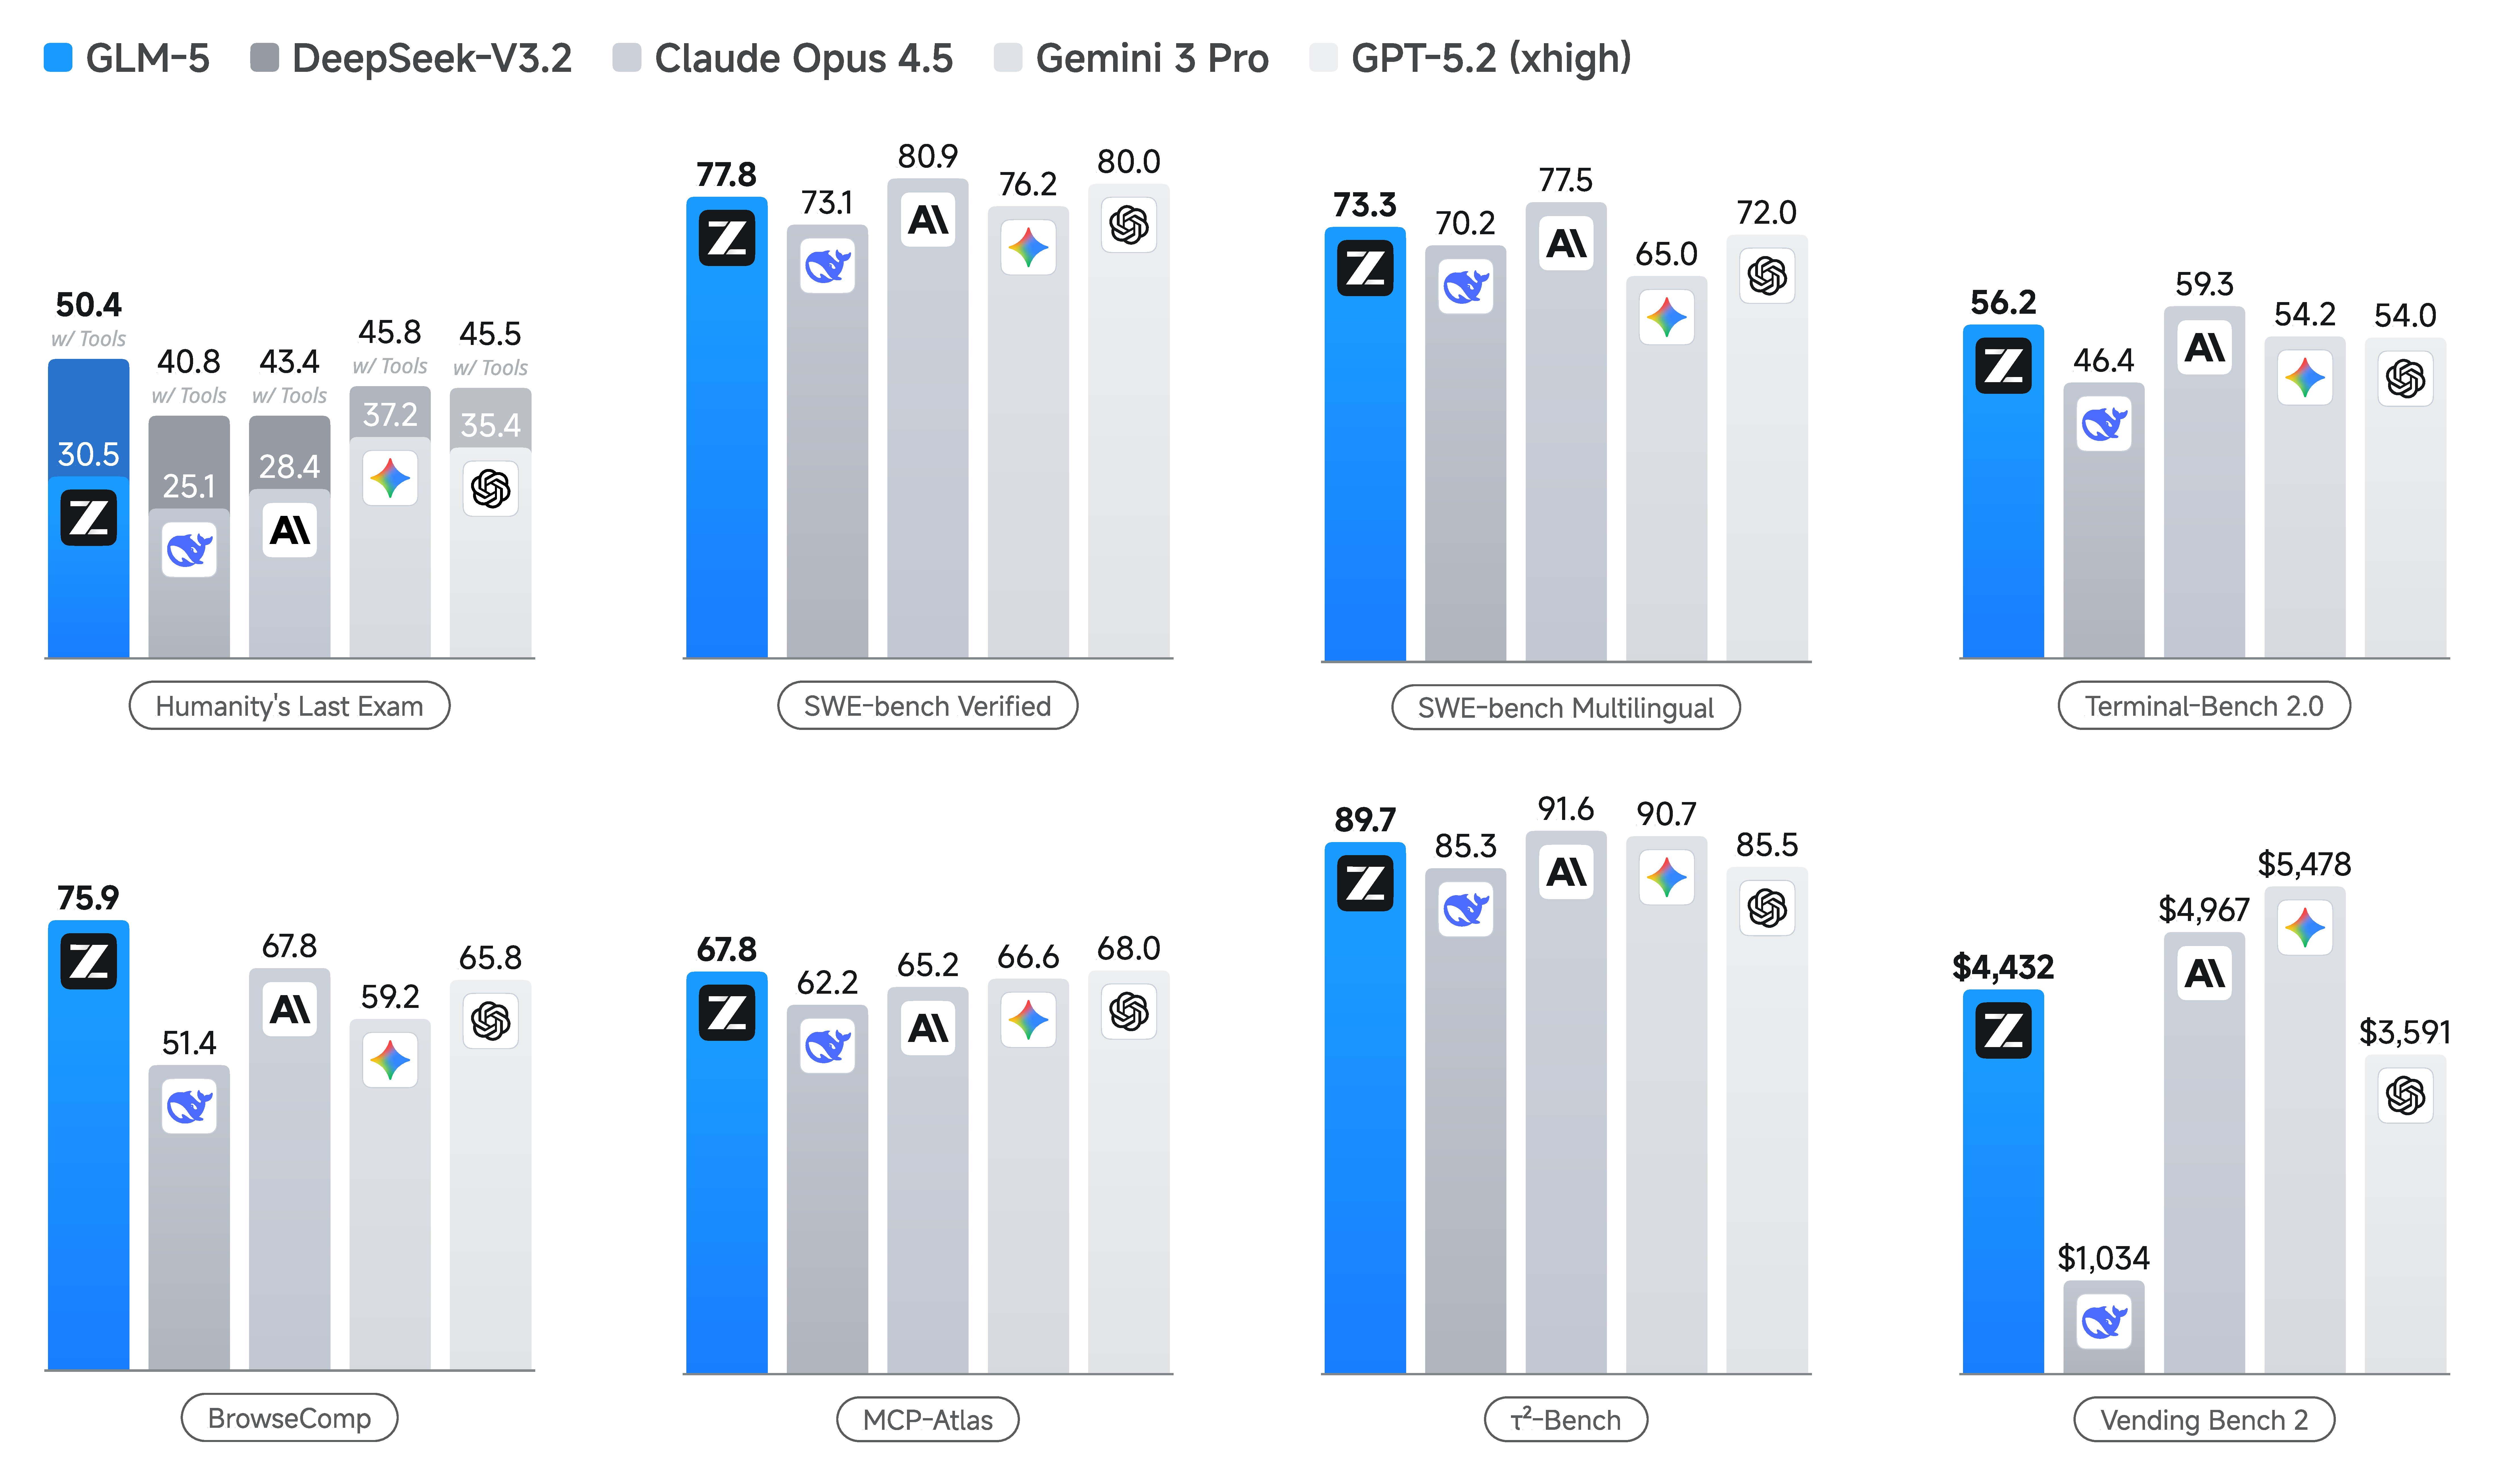
\includegraphics[width=\linewidth]{figures/arc_clean.pdf}
    \caption{Results of GLM-5, DeepSeek-V3.2, Claude Opus 4.5, Gemini 3 Pro, and GPT-5.2 (xhigh) on 8 agentic, reasoning, and coding benchmarks: Humanity's Last Exam, SWE-bench Verified, SWE-bench Multilingual, Terminal-Bench 2.0, BrowseComp, MCP-Atlas, $\tau^2$-Bench, Vending Bench~2.}
    \label{fig:arc}
\end{figure}


\section{Introduction}

The pursuit of Artificial General Intelligence (AGI) requires not only scaling model parameters but also fundamentally rethinking the efficiency of intelligence and the architecture of autonomous improvement. With the release of GLM-4.5, we demonstrated that uniting Agentic, Reasoning, and Coding (ARC) capabilities into a single Model-of-Experts (MoE) architecture could yield state-of-the-art results across diverse benchmarks. However, as Large Language Models (LLMs) transition from passive knowledge repositories to active problem solvers, the dual challenges of computational cost and real-world adaptability—particularly in complex software engineering—have become the primary bottlenecks.

We present GLM-5, our next-generation flagship model designed to overcome these barriers. GLM-5 represents a paradigm shift in both performance and efficiency, achieving state-of-the-art status on major open leaderboards, including ArtificialAnalysis.ai, the LMArena Text, and the LMArena Code. More significantly, GLM-5 redefines the standard for real-world coding, demonstrating an unprecedented ability to handle complex, end-to-end software development tasks that go far beyond the scope of traditional static benchmarks like SWE-bench.

\paragraph{Results.} Figure~\ref{fig:arc} shows the results of GLM-5, GLM-4.7, Claude Opus 4.5, Gemini 3 Pro, and GPT-5.2 (xhigh) on 8 agentic, reasoning, and coding benchmarks: Humanity's Last Exam~\cite{phan2025humanity}, SWE-bench Verified~\cite{jimenez2023swe}, SWE-bench Multilingual~\cite{yang2025swemulti}, Terminal-Bench 2.0~\cite{tbench_2025}, BrowseComp~\cite{wei2025browsecomp}, MCP-Atlas~\cite{bandi2026mcp}, $\tau^2$-Bench~\cite{yao2024tau,barres2025tau2}, Vending Bench 2~\cite{backlund2025vending}. On average, GLM-5 achieves about 20\% improvement over our last version GLM-4.7, and is comparable to Claude Opus 4.5 and GPT-5.2 (xhigh), and better than Gemini 3 Pro.

GLM-5 scores 50 on the Intelligence Index v4.0 and is the new open weights leader (Cf. Figure~\ref{fig:aa}), up from GLM-4.7's score of 42 - an 8 point jump driven by improvements across agentic performance and knowledge/hallucination. This is the first time an open weights model has achieved a score of 50 on the Artificial Analysis Intelligence Index v4.0.

\begin{figure}[t]
    \centering
    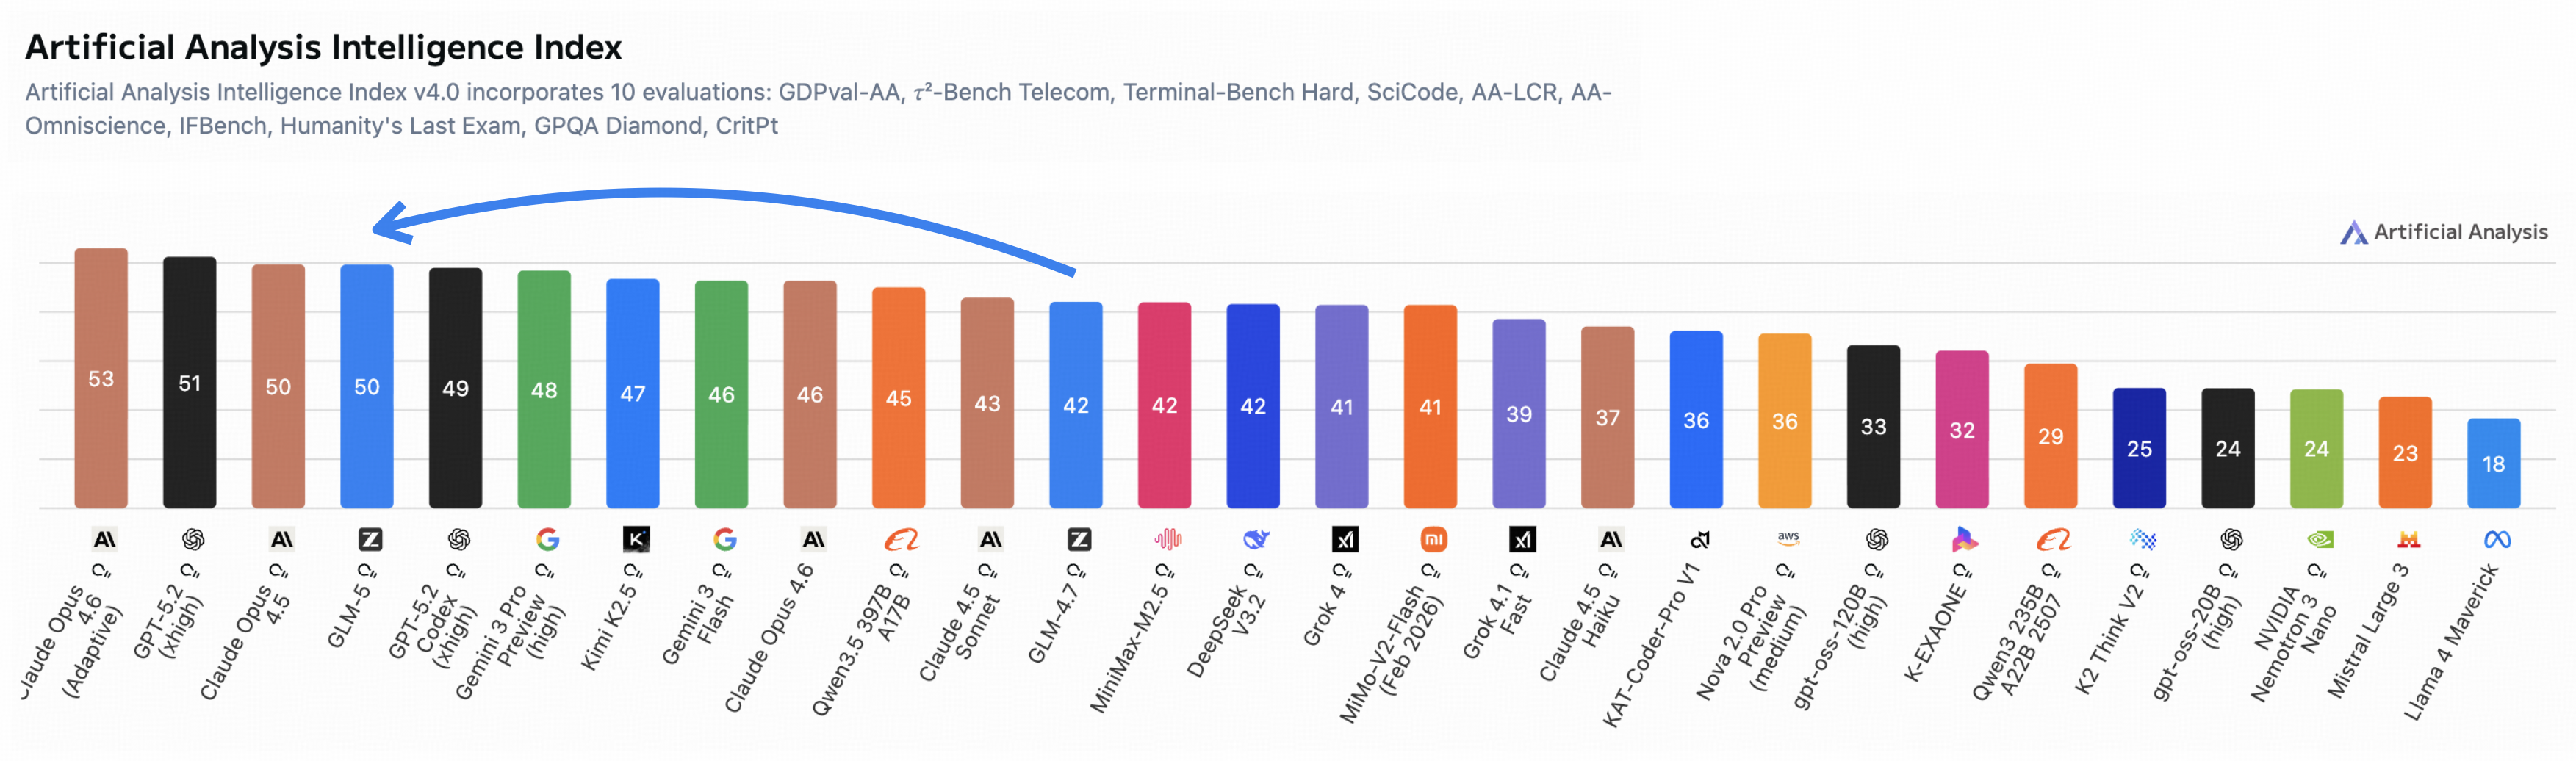
\includegraphics[width=1\linewidth]{figures/aa.PNG}
    \caption{Artificial Analysis Intelligence Index v4.0 incorporates 10 evaluations: GDPval-AA, $\tau^2$-Bench Telecom, Terminal-Bench Hard, SciCode, AA-LCR, AA-Omniscience, IFBench, Humanity's Last Exam, GPQA Diamond, CritPt.}
    \label{fig:aa}
\end{figure}

\begin{figure}[t]
    \centering
    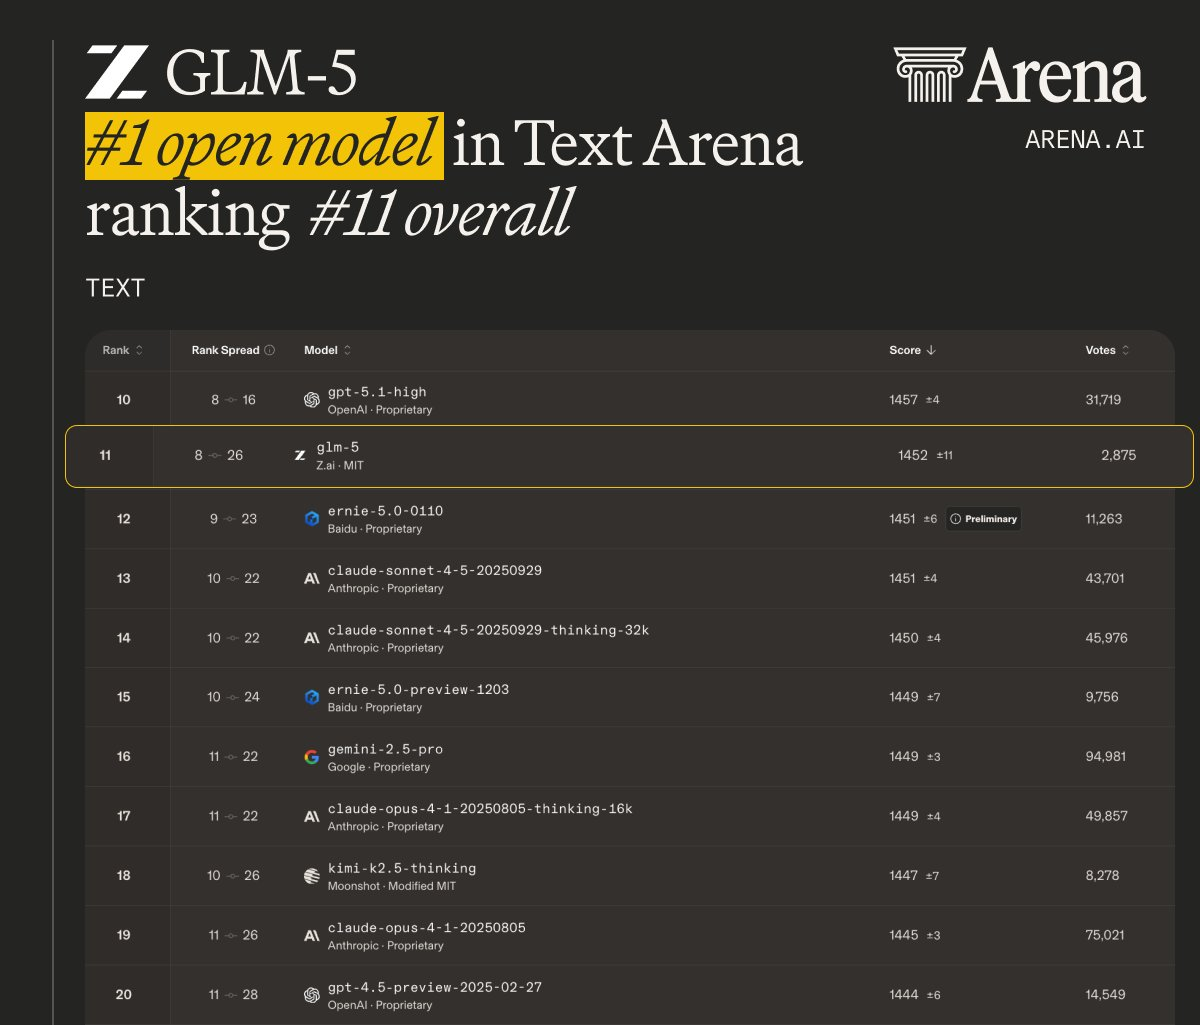
\includegraphics[width=0.48\linewidth]{figures/text-arena.jpeg} \;\;\;
    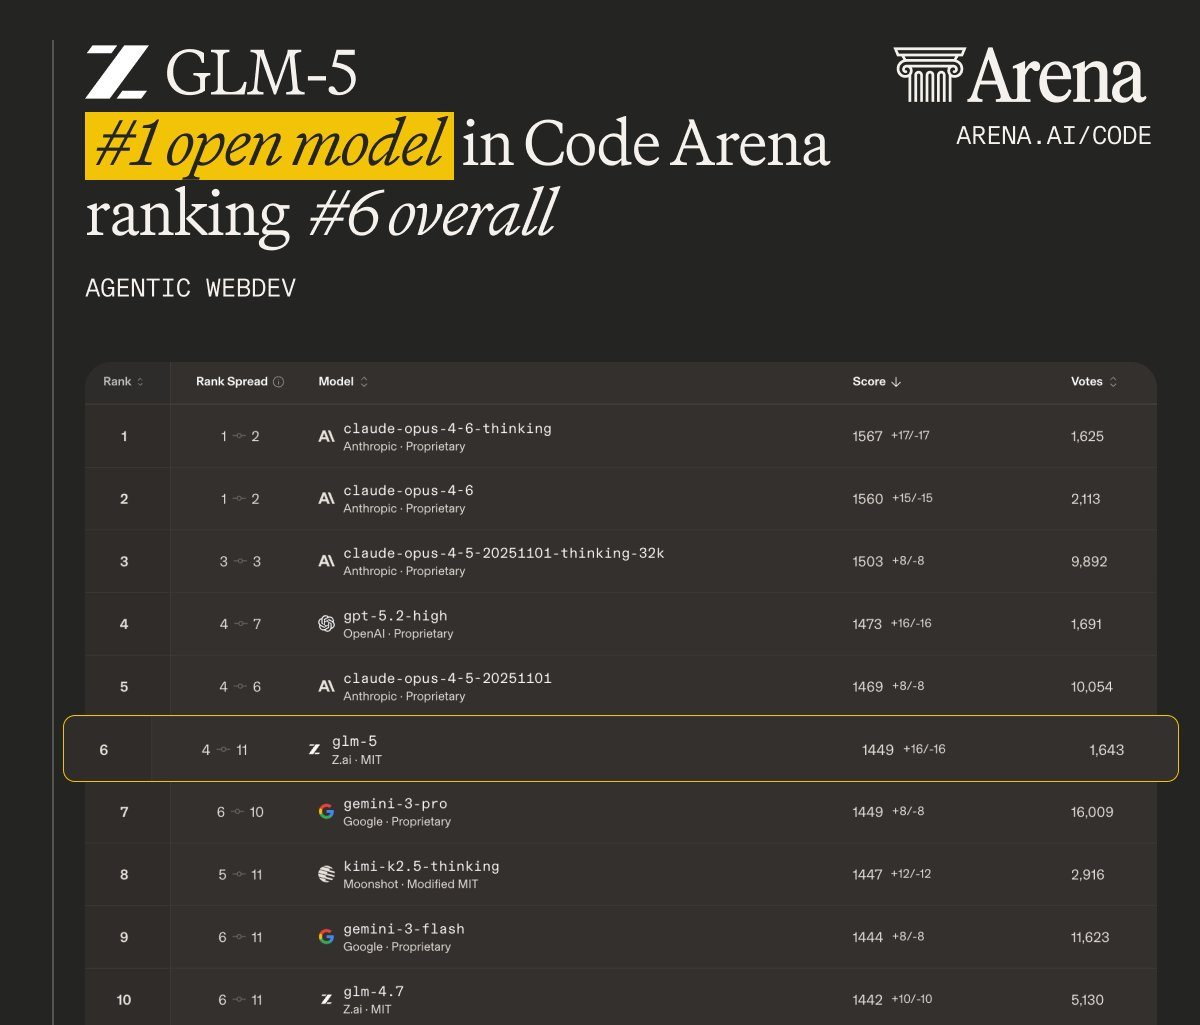
\includegraphics[width=0.48\linewidth]{figures/code-arena.jpeg}
    \caption{On LMArena, GLM-5 is the \#1 open model in both Text Arena and Code Arena.}
    \label{fig:arena}
\end{figure}

\begin{figure}[t]
    \centering
    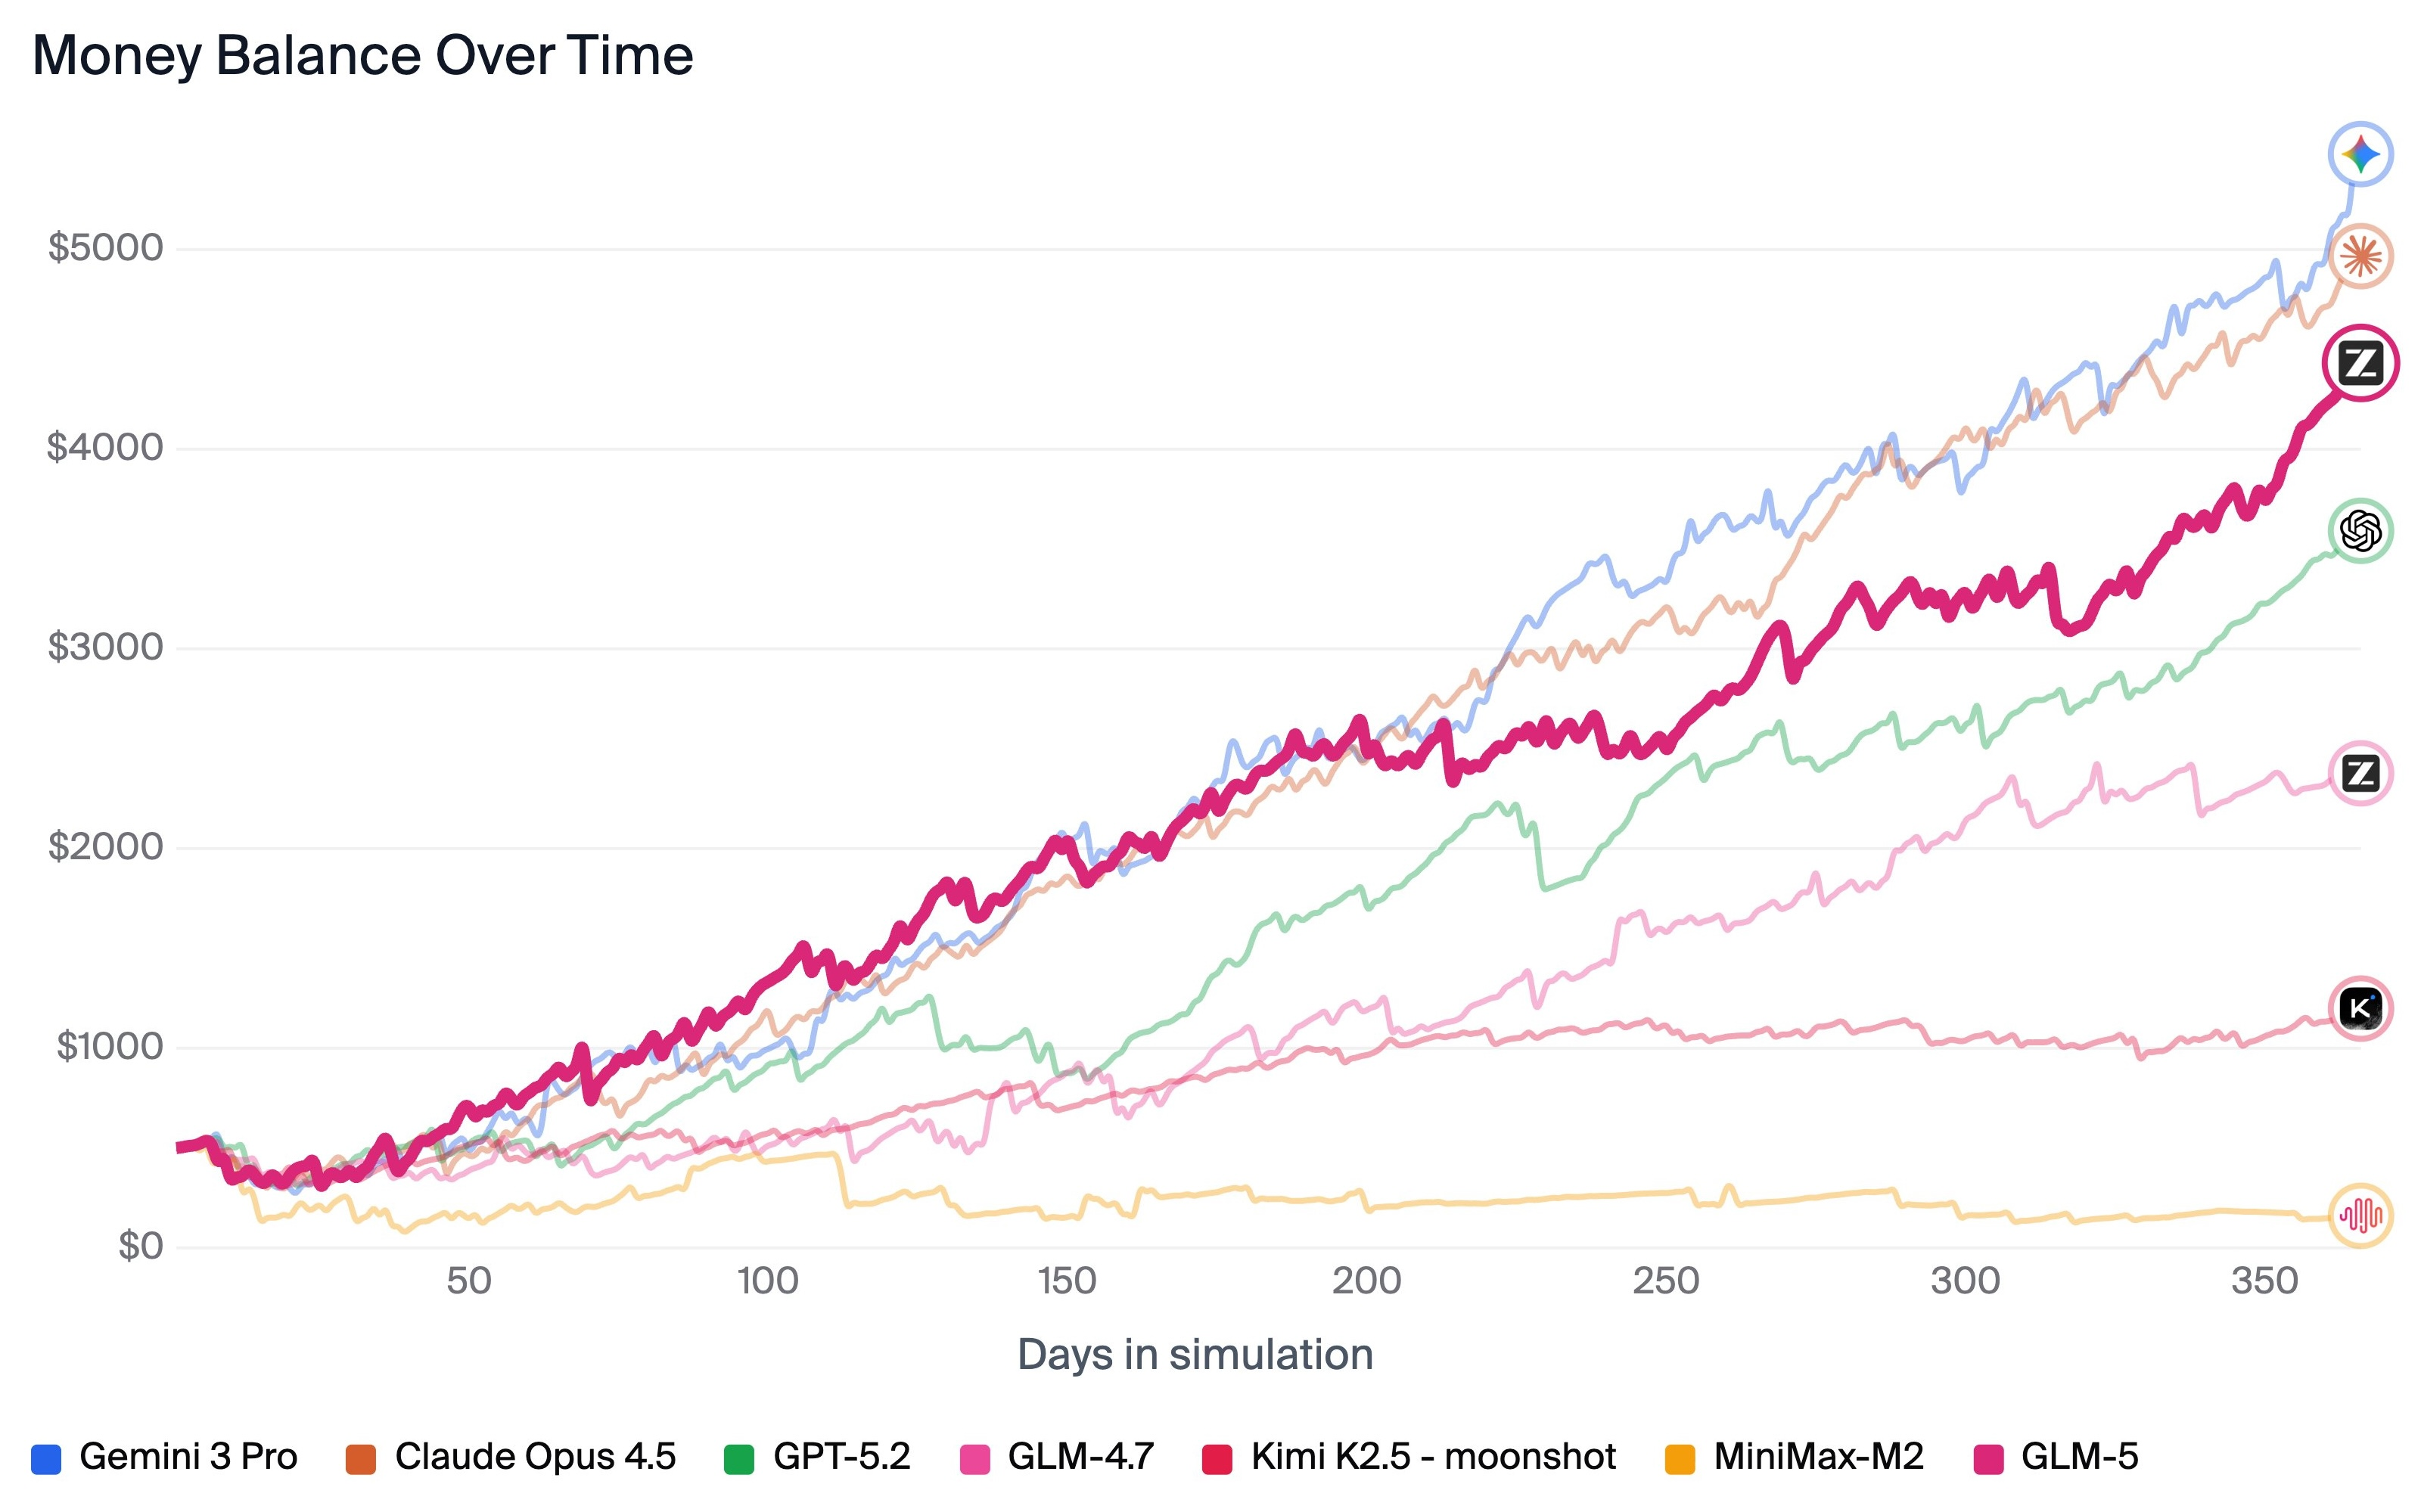
\includegraphics[width=0.50\linewidth]{figures/vending-bench.jpeg} \;\;
    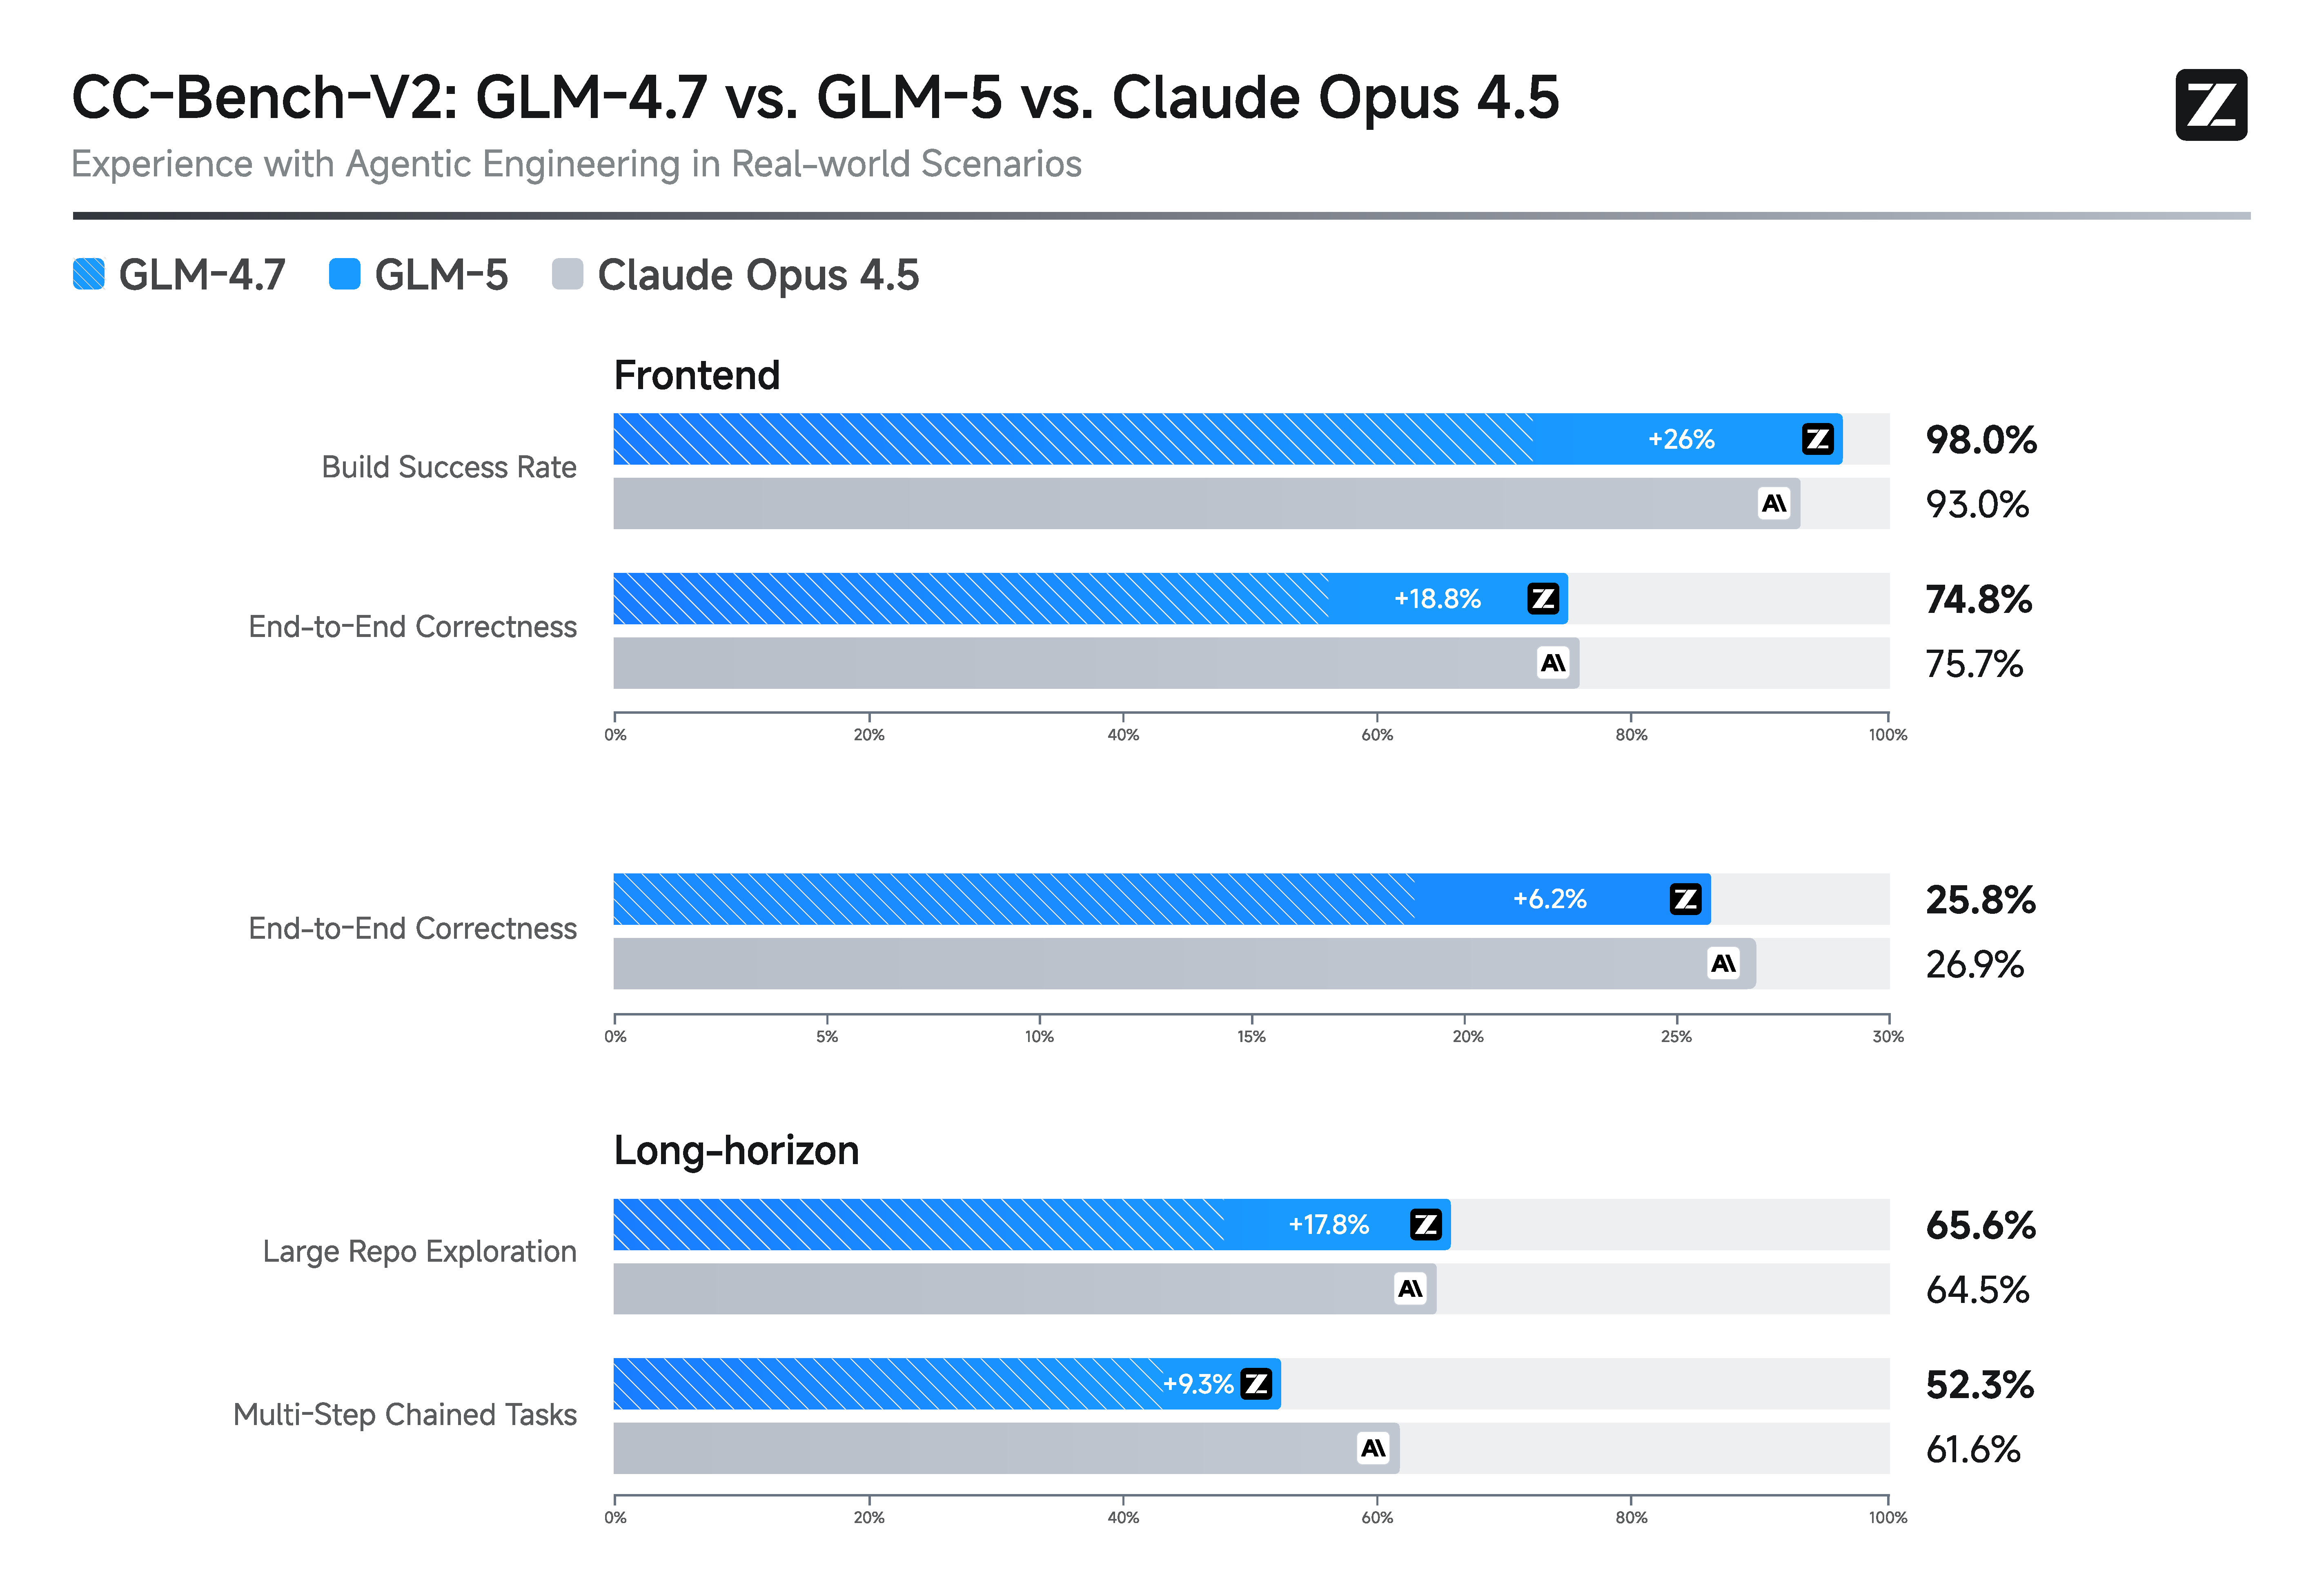
\includegraphics[width=0.47\linewidth]{figures/cc-bench-v2.pdf}
    \caption{Results on several long-horizon tasks. Left: Vending-Bench 2; Right: CC-Bench-V2.}
    \label{fig:vendingcc}
\end{figure}

LMArena, initiated by UC Berkeley, is a transparent, shared space to evaluate and compare frontier AI capabilities by human judgment with millions of real tasks, including writing, coding, reasoning, designing, searching, and creating. The large volume of human interactions generates signals of real-world utility, making it different from the other static benchmarks.
Figure~\ref{fig:arena} shows that GLM-5 again is the \#1 open model in both Text Arena and Code Arena, and overall 
on par with Claude-Opus-4.5 and Gemini-3-pro.


Long-term coherence in agents becomes more and more important. Coding agents can now write code autonomously for hours, and the length and breadth of tasks AI models are able to complete are likely to increase. We use two benchmarks, Vending-Bench 2 and CC-Bench-V2, to evaluate how GLM-5 is able to complete long-horizon tasks.
Vending-Bench 2 is a benchmark for measuring AI model performance in running a business over long time horizons. Models are tasked with running a simulated vending machine business over a year and are scored on their bank account balance at the end.
Figure~\ref{fig:vendingcc} (left) shows that GLM-5 ranks \#1 among all open-source models, finishing with a final account balance of \$4,432. It approaches Claude Opus 4.5, demonstrating strong long-term planning and resource management.
Figure~\ref{fig:vendingcc} (right) further shows results on our internal evaluation suite CC-Bench-V2. GLM-5 significantly outperforms GLM-4.7 across frontend, backend, and long-horizon tasks, narrowing the gap with Claude Opus 4.5.


\begin{figure}[t]
    \centering
    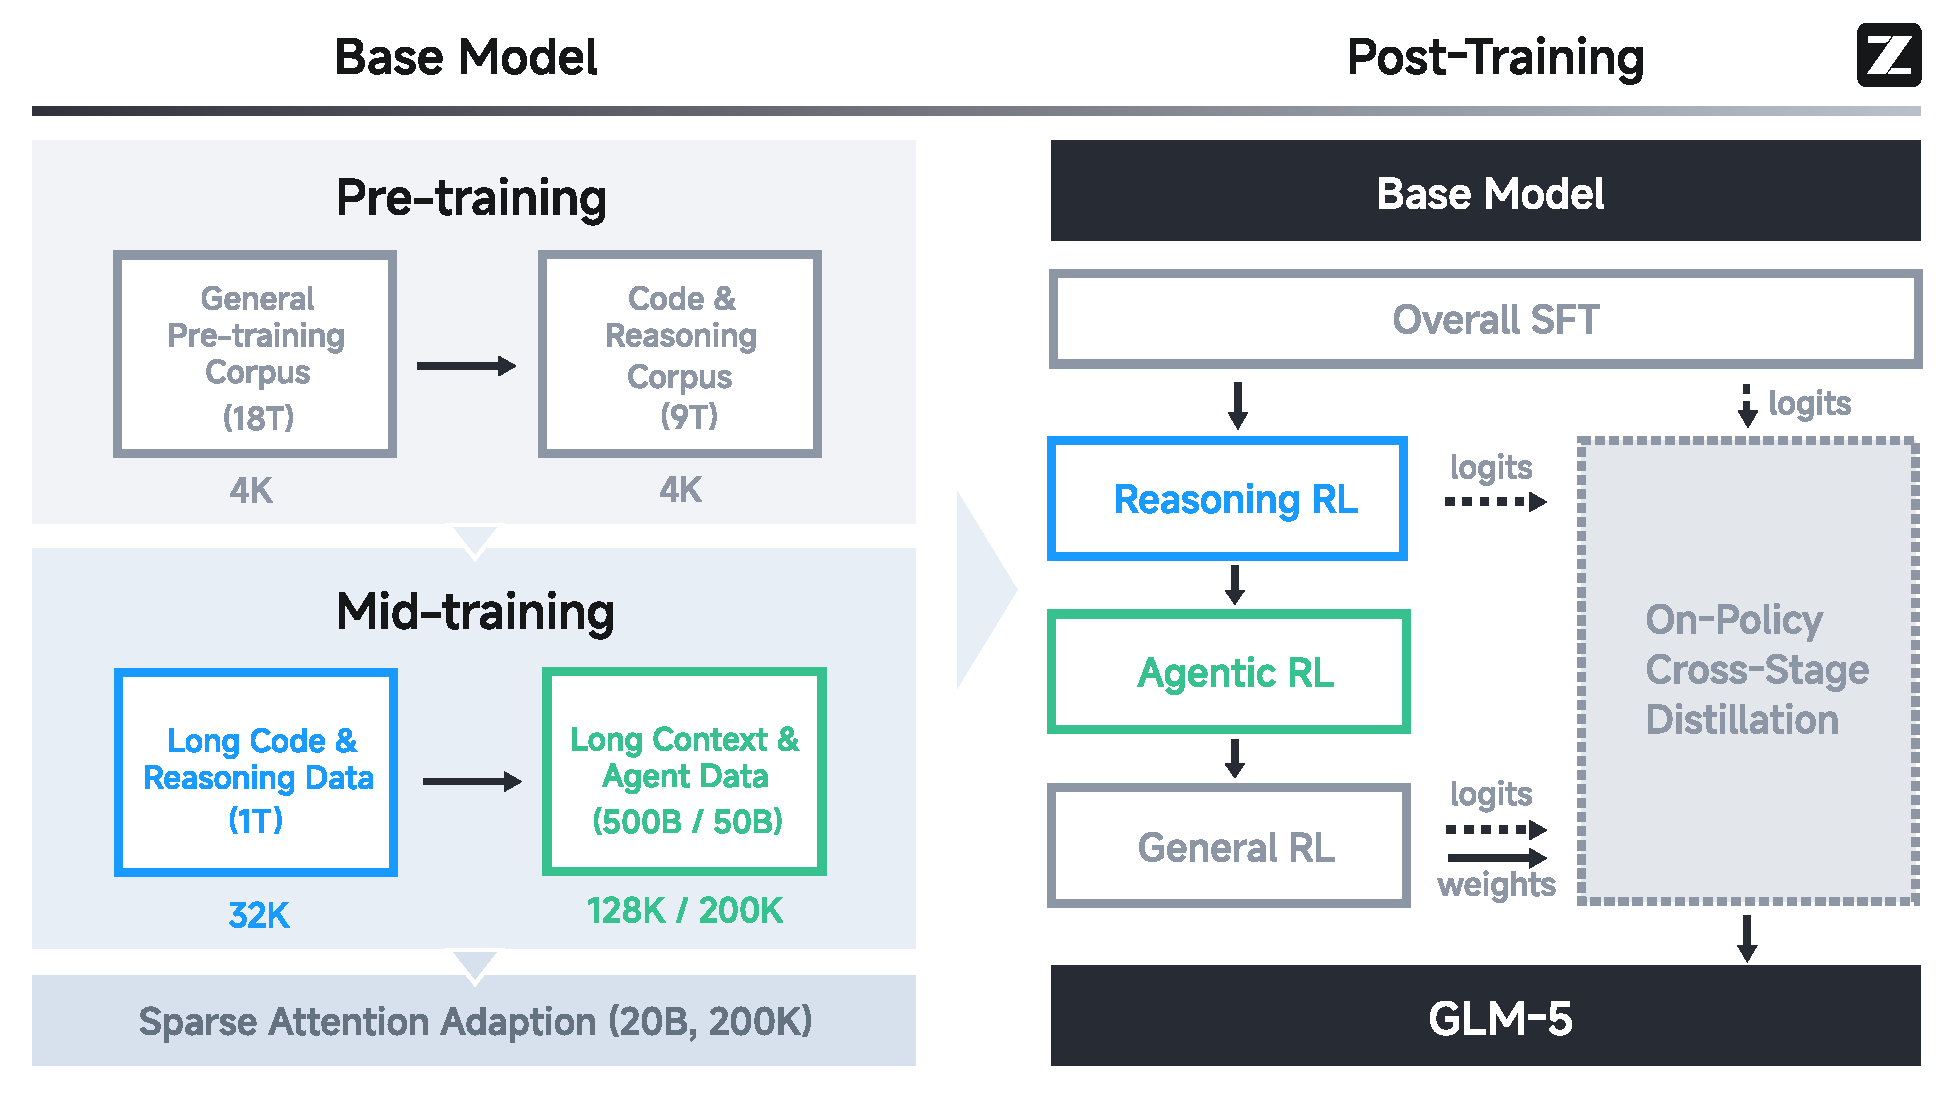
\includegraphics[width=1\linewidth]{figures/overall_pipeline.pdf}
    \caption{Overall training pipeline of GLM-5.}
    \label{fig:overall_pipeline}
\end{figure}

\paragraph{Methods.} Figure~\ref{fig:overall_pipeline} shows the overall training pipeline of GLM-5.
Our Base Model training began with a massive 27 trillion token corpus, prioritizing code and reasoning early on. We then employed a distinct Mid-training phase to progressively extend context length from 4K to 200K, focusing specifically on long-context agentic data to ensure stability in complex workflows.
In Post-Training, we moved beyond standard SFT. We implemented a sequential Reinforcement Learning pipeline—starting with Reasoning RL, followed by Agentic RL, and finishing with General RL. Crucially, we utilized On-Policy Cross-Stage Distillation throughout this process to prevent catastrophic forgetting, ensuring the model retains its sharp reasoning edge while becoming a robust generalist.
In summary, the leap in GLM-5’s performance is driven by the following technical contributions:

First, we adopt DSA (DeepSeek Sparse Attention)~\cite{deepseekai2025deepseekv32pushingfrontieropen}, a novel architectural innovation that significantly reduces both training and inference costs. While GLM-4.5 improved efficiency through a standard MoE architecture, DSA allows GLM-5 to dynamically allocate attention resources based on token importance, drastically lowering the computational overhead without compromising long-context understanding or reasoning depth. With DSA, we scale the model parameters up to 744B and extend the training token budget to ~28.5T tokens.

Second, we have engineered a new asynchronous reinforcement learning infrastructure. Building on the ``slime'' framework and the decoupled rollout engines initialized in GLM-4.5, our new infrastructure further decouples generation from training to maximize GPU utilization. This system allows for massive-scale exploration of agent trajectories without the synchronization bottlenecks that previously hampered iteration speed, significantly improving the efficiency of our RL post-training pipeline.

Third, we present novel asynchronous Agent RL algorithms designed to enhance the quality of autonomous decision-making. In GLM-4.5, we utilized iterative self-distillation and outcome supervision to train agents. For GLM-5, we have developed asynchronous algorithms that allow the model to learn from diverse, long-horizon interactions continuously. These algorithms are specifically optimized to improve the model's planning and self-correction capabilities in dynamic environments, directly contributing to our dominance in real-world coding scenarios.

Last, one more technical contribution lies in the fact that, from the first day, GLM-5 is full-stack adapted to Chinese GPU ecosystems. We have successfully completed deep optimization—spanning from underlying kernels to upper-level inference frameworks—across seven mainstream domestic chip platforms, including Huawei Ascend, Moore Threads, Hygon, Cambricon, Kunlunxin, MetaX, and Enflame.

With these advancements, GLM-5 stands not just as a more powerful model but as a more efficient and practical foundation for the next generation of AI agents. We release GLM-5 to the community to further advance the frontier of efficient, agentic general intelligence.
